\documentclass[a4paper, 10pt, final]{article}

\usepackage{a4wide}

\usepackage{charter}
\usepackage{verbatim}
\usepackage{amsfonts}
\usepackage{amsmath}
\usepackage{amsthm}
\usepackage{amssymb}
%\usepackage[integrals]{wasysym}
%\usepackage{mathrsfs}
%\usepackage[mathcal]{euscript}
\usepackage{listings}
\usepackage{graphicx}
\usepackage{multirow}
\usepackage{hyperref}
\usepackage{float}
\usepackage[small,bf]{caption}
%\usepackage{xypic}
\usepackage[table]{xcolor}
\usepackage{subfig}
%\usepackage{ulem} %use \normalem after begin document
\usepackage[authoryear]{natbib}

% Settings
\parindent=5pt
\parskip=8pt plus 2pt minus 4pt
\lstset{language=Matlab, basicstyle=\scriptsize,
    showstringspaces=false, numbers=left, stepnumber=1, numberstyle=\tiny, frame=tb}


%% \def\mytitle{Signal and Image Processing 2010}
%% \def\mysubtitle{Handin of mandatory excercise 1}
%% \def\myauthor{Ulrik Bonde}
%% \def\mymail{\mailto{bonde@diku.dk}}
%% \def\mydate{\today}

\title{Statistical Methods for Machine Learning \\ Mandatory Project 1}
\author{Kasper Steenstrup \& Michael Andersen}
\date{\today}

%% \title{\mytitle}
%% \subtitle{\mysubtitle}

%% \author{\myauthor{} - \mymail}
%% \date{\mydate}

\hypersetup{
colorlinks,%
citecolor=black,%
filecolor=black,%
linkcolor=black,%
urlcolor=black,%
bookmarksopen=false,
pdftitle={Statistical Methods for Machine Learning - Mandatory Project 1},
pdfauthor={Kasper Steenstrup \& Michael Andersen}
}

\begin{document}
\maketitle

\subsection*{Question 1.1 and 1.2}

In figure \ref{fig:q1_1} can be seen the $100$ data points drawn from
the gaussian distribution with $\mu = [1.0~ 1.0]$ and $\Sigma = [0.3~
  0.2; 0.2~ 0.2]$. The correct $\mu$ is blue and $\widehat{\mu}$ is
marked with red. The code can be seen in \ref{text:Code}

\begin{figure}[!ht]
  \centering
  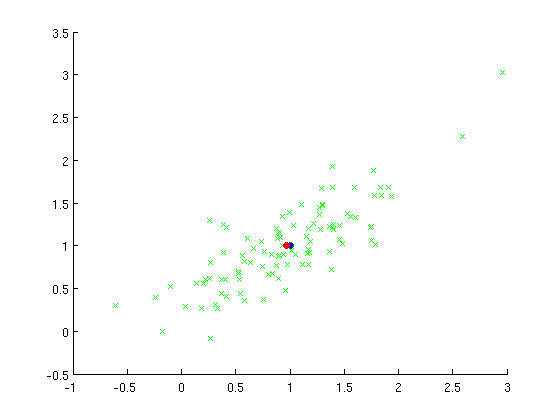
\includegraphics[width=0.6\textwidth]{images/q1_1}
  \caption{100 data points, correct mean with blue and estimated mean red.}
  \label{fig:q1_1}
\end{figure}

To quantify how much the estimated mean deviates from the correct
mean, we use usual euclidean distance between the two vectors.

Our distance is $0.0392$, which is not very much. This can also be
seen from the drawing, the points are placed really close.

\subsection*{Question 1.3}

\begin{figure}[!ht]
  \centering
  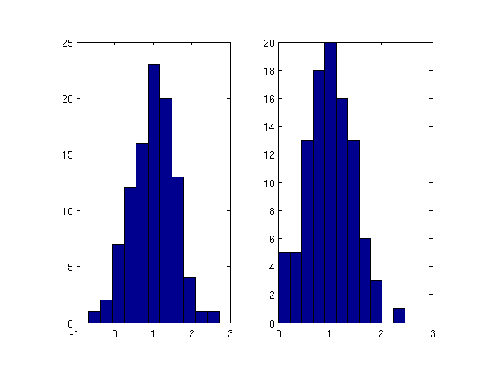
\includegraphics[width=0.6\textwidth]{images/q1_3a}
  \caption{a shows $p(x_1)$ and b shows $p(x_2)$ using 11 bins.}
  \label{fig:q1_3a}
\end{figure}

\begin{figure}[!ht]
  \centering
  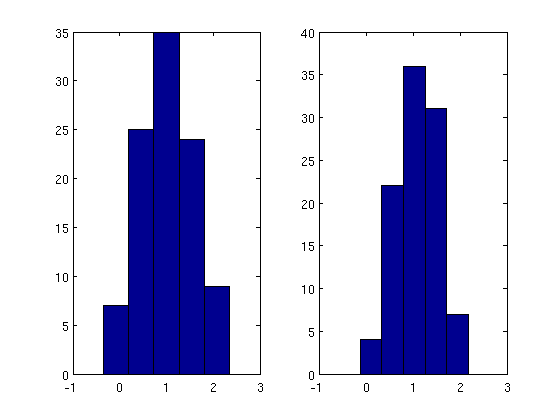
\includegraphics[width=0.6\textwidth]{images/q1_3b}
  \caption{a shows $p(x_1)$ and b shows $p(x_2)$ using 5 bins.}
  \label{fig:q1_3b}
\end{figure}

\begin{figure}[!ht]
  \centering
  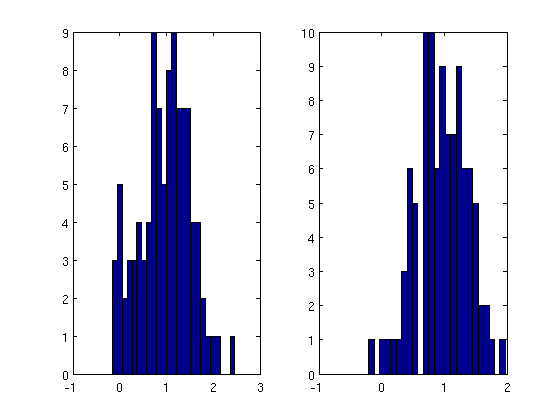
\includegraphics[width=0.6\textwidth]{images/q1_3c}
  \caption{a shows $p(x_1)$ and b shows $p(x_2)$ using 25 bins.}
  \label{fig:q1_3c}
\end{figure}

There is no best way to select the bin width. If it is selected too
small, the resulting density becomes very spiky and unable to capture
the structure of the distribution. Selecting the bin width too large,
can result in bimodal structure of the distribution being lost. So one
needs to use some intermediate value as bin width. In our case,
selecting a total of 11 bins seems to provide a good estimation of the
distribution.

\subsection*{Question 1.4}

From the figures it can be seen that the gaussian distribution is
rotated because the $\Sigma$-matrix different values in the
diagonal. The figures show the same tendency as in question 1.3 and
can be solved by looking at the figures and selecting appropriate bin
numbers.

\begin{figure}[!ht]
  \centering
  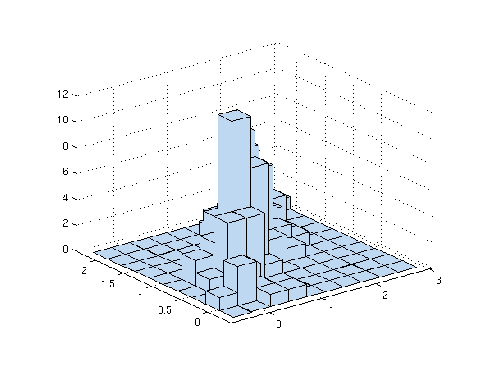
\includegraphics[width=0.6\textwidth]{images/q1_4_100}
  \caption{Shows 3d histogram of 100 datapoints using $10$x$10$ bins}
  \label{fig:q1_4_100}
\end{figure}

\begin{figure}[!ht]
  \centering
  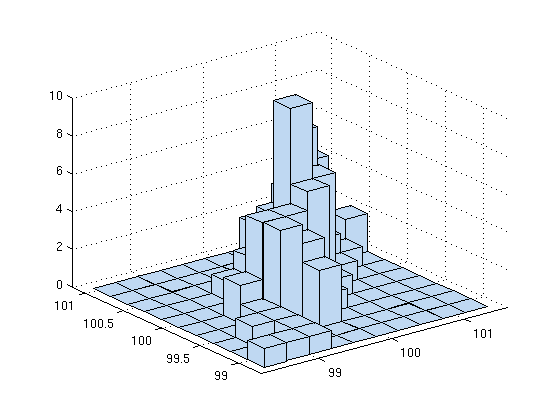
\includegraphics[width=0.6\textwidth]{images/q1_4_1000}
  \caption{Shows 3d histogram of 1000 datapoints using $10$x$10$ bins}
  \label{fig:q1_4_1000}
\end{figure}

\begin{figure}[!ht]
  \centering
  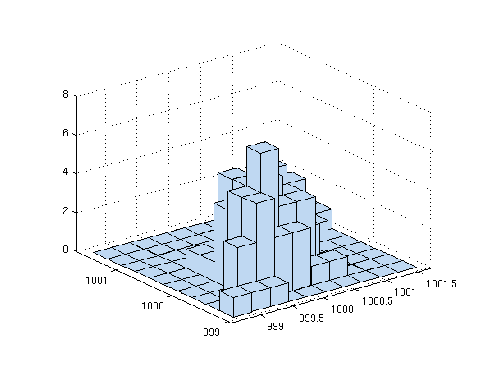
\includegraphics[width=0.6\textwidth]{images/q1_4_10000}
  \caption{Shows 3d histogram of 10000 datapoints using $10$x$10$ bins}
  \label{fig:q1_4_10000}
\end{figure}

\begin{figure}[!ht]
  \centering
  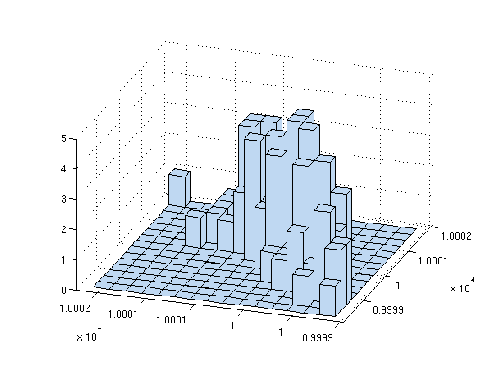
\includegraphics[width=0.6\textwidth]{images/q1_4_10000_b15}
  \caption{Shows 3d histogram of 10000 datapoints using $15$x$15$ bins}
  \label{fig:q1_4_10000_b15}
\end{figure}

\begin{figure}[!ht]
  \centering
  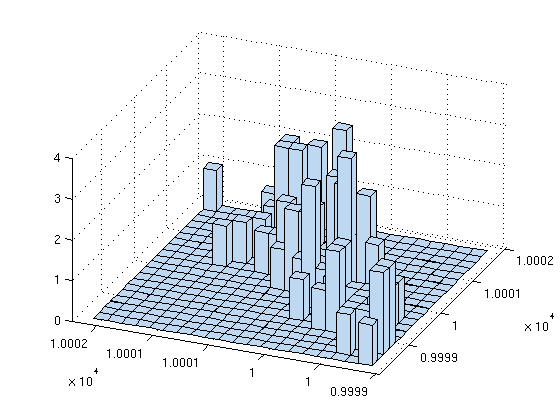
\includegraphics[width=0.6\textwidth]{images/q1_4_10000_b20}
  \caption{Shows 3d histogram of 10000 datapoints using $20$x$20$ bins}
  \label{fig:q1_4_10000_b20}
\end{figure}


%% \begin{figure}
%% \centering
%% \subfloat[]{\includegraphics[width=0.3\textwidth]{images/img00}}
%% \subfloat[]{\includegraphics[width=0.45\textwidth]{images/img00h}}
%% \caption{Original image and histogram, unadjusted}
%% \label{fig:original}
%% \end{figure}

\newpage
\subsection*{\label{text:Code}}
\lstinputlisting{../src/probability_and_parameter_estimation.m}


%%%%%%%%%%%%%%%%%%%%%%%%%%%%%%%%%%%%%%%%%%%%%%%%%%%%%%%%%%%%%%%%%%%%
% Formal stuff

%\bibliographystyle{abbrvnat}
%\bibliography{bibliography}
%\addcontentsline{toc}{chapter}{Litteratur}

\end{document}

% vim: set tw=72 spell spelllang=en:
